%%%%%%%%%%%%%%%%%%%%%%%%%%%%%%%%%%%%%%%%%%%%%%%%%%%%%%%%%%%%%%%%%%%%%%%%%%%%%%%%%%
\begin{frame}[fragile]\frametitle{}
\begin{center}
{\Large Installations}
\end{center}
\end{frame}

%%%%%%%%%%%%%%%%%%%%%%%%%%%%%%%%%%%%%%%%%%%%%%%%%%%%%%%%%%%%%%%%%%%%%%%%%%%%%%%%%%%
\begin{frame}[fragile]\frametitle{Installing Python}
  \begin{itemize}
  \item Pre-installed on most Unix, Linux and MAC OS X
   \item Windows: Python.org or Anaconda (preferred)
   \item Anaconda has necessary libraries
\item 2.* and 3.* both
\item `pip' and `conda'
  \end{itemize}
\end{frame}

%%%%%%%%%%%%%%%%%%%%%%%%%%%%%%%%%%%%%%%%%%%%%%%%%%%%%%%%%%%%%%%%%%%%%%%%%%%%%%%%%%%
\begin{frame}[fragile]\frametitle{Installing Python by Anaconda Distribution}
  \begin{itemize}
  \item Need Python 3.5 (not 2.* or 3.6)
  \item By default in Anaconda 4.2.0
  \item Site: https://repo.continuum.io/archive/
  \item 64 Bit: Anaconda3-4.2.0-Windows-x86\_64.exe
  \item 32 bit: Anaconda3-4.2.0-Windows-x86.exe
  \item About 300+MB
  \end{itemize}
\end{frame}

%%%%%%%%%%%%%%%%%%%%%%%%%%%%%%%%%%%%%%%%%%%%%%%%%%%%%%%%%%%%%%%%%%%%%%%%%%%%%%%%%%%
\begin{frame}[fragile]  \frametitle{The Python shell, I}
  \begin{itemize}
 \item Can run from ``shell'', IDE, Notebook
 \item Shell/Command Line:
\begin{lstlisting}
$ python

Python 3.5.3 | packaged by conda-forge | (default, May 12 2017, 16:16:49) [MSC v.1900 64 bit (AMD64)] on win32
Type "help", "copyright", "credits" or "license" for more information.
>>>
\end{lstlisting}
\item Start typing at  $>>>$ 
\end{itemize}
\end{frame}

%%%%%%%%%%%%%%%%%%%%%%%%%%%%%%%%%%%%%%%%%%%%%%%%%%%%%%%%%%%%%%%%%%%%%%%%%%%%%%%%%%%
\begin{frame}[fragile]  \frametitle{The Python shell, I}
  \begin{itemize}
 \item Typing anything??
\begin{lstlisting}
>>> I come in peace, please take me to your leader
File "<stdin>" , line 1
I come in peace, please take me to your leader
^
SyntaxError : invalid syntax
>>>
\end{lstlisting}
\item Need to learn syntax
\end{itemize}
\end{frame}

%%%%%%%%%%%%%%%%%%%%%%%%%%%%%%%%%%%%%%%%%%%%%%%%%%%%%%%%%%%%%%%%%%%%%%%%%%%%%%%%%%%
\begin{frame}[fragile]\frametitle{The Python shell, II}
\begin{itemize}
\item Expressions: evaluated, result printed:
\begin{lstlisting}
>>> 2+2
4
\end{lstlisting}
\item Line continuation \\ 
\begin{lstlisting}
>>> "hello" + \
... " world!"
'hello world!'
\end{lstlisting}
\item Prompt changes to `\texttt{...}' on continuation lines.
\end{itemize}
\end{frame}

%%%%%%%%%%%%%%%%%%%%%%%%%%%%%%%%%%%%%%%%%%%%%%%%%%%%%%%%%%%%%%%%%%%%%%%%%%%%%%%%%%%
\begin{frame}[fragile]\frametitle{The Python shell, II}
\begin{itemize}
\item Syntactically correct:
	\begin{lstlisting}
>>>print('I come in peace, please take me')
	\end{lstlisting}

\item \lstinline|print| is a function, with defined syntax. 
\item If you don't obey: \\ 
\begin{lstlisting}
>>>print 'I come in peace, please take me'
File "<stdin>", line 1
print 'I come in peace, please take me'
^
SyntaxError: Missing parentheses in call to 'print'
\end{lstlisting}
\end{itemize}
\end{frame}

%%%%%%%%%%%%%%%%%%%%%%%%%%%%%%%%%%%%%%%%%%%%%%%%%%%%%%%%%%%%%%%%%%%%%%%%%%%%%%%%%%%
\begin{frame}[fragile]\frametitle{The Python shell, II}
\begin{itemize}
\item To exit:
	\begin{lstlisting}
>>> good-bye
Traceback (most recent call last):
File"<stdin>", line1, in <module>
NameError name 'good' is not defined
>>> if you don't mind, I need to leave 
File "<stdin>", line 1
if you don't mind, I need to leave
          ^
SyntaxError: invalid syntax
	\end{lstlisting}

\item Better to: \\ 
\begin{lstlisting}
>>> quit()
\end{lstlisting}
\end{itemize}
\end{frame}

%%%%%%%%%%%%%%%%%%%%%%%%%%%%%%%%%%%%%%%%%%%%%%%%%%%%%%%%%%%%%%%%%%%%%%%%%%%%%%%%%%%
\begin{frame}[fragile]\frametitle{Exercises}
\begin{itemize}
\item Find more about JIT-compilation.
\item Install any IDE, having debugging.
\item Get familiar with command prompt.
\end{itemize}
\end{frame}

%%%%%%%%%%%%%%%%%%%%%%%%%%%%%%%%%%%%%%%%%%%%%%%%%%%%%%%%%%%%%%%%%%%%%%%%%%%%%%%%%%%
\begin{frame}[fragile]\frametitle{Integrated Dev Envt}
  \begin{itemize}
  \item Pycharm https://www.jetbrains.com/pycharm/
  \item IDLE comes with python.org distribution
  \item Spyder https://pypi.python.org/pypi/spyder
  \end{itemize}
\end{frame}

%%%%%%%%%%%%%%%%%%%%%%%%%%%%%%%%%%%%%%%%%%%%%%%%%%%%%%%%%%%%%%%%%%%%%%%%%%%%%%%%%%%
\begin{frame}[fragile]\frametitle{PyCharm}
Download the community edition of Pycharm
\begin{center}
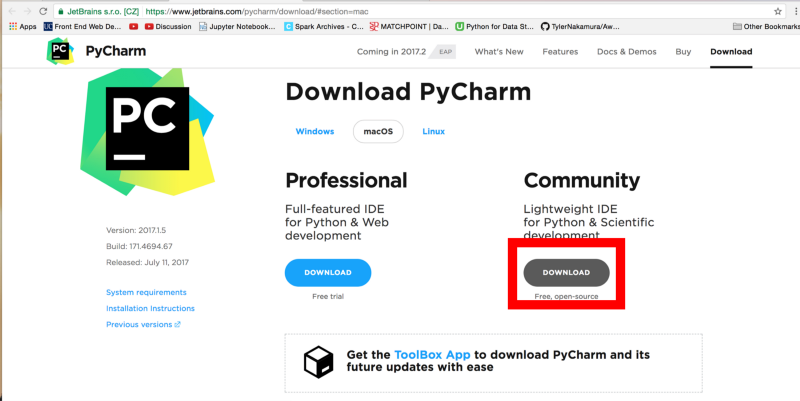
\includegraphics[width=0.7\linewidth,keepaspectratio]{pycharm1}
\end{center}
\end{frame}

%%%%%%%%%%%%%%%%%%%%%%%%%%%%%%%%%%%%%%%%%%%%%%%%%%%%%%%%%%%%%%%%%%%%%%%%%%%%%%%%%%%
\begin{frame}[fragile]\frametitle{PyCharm Project}
Create a New Project
\begin{center}
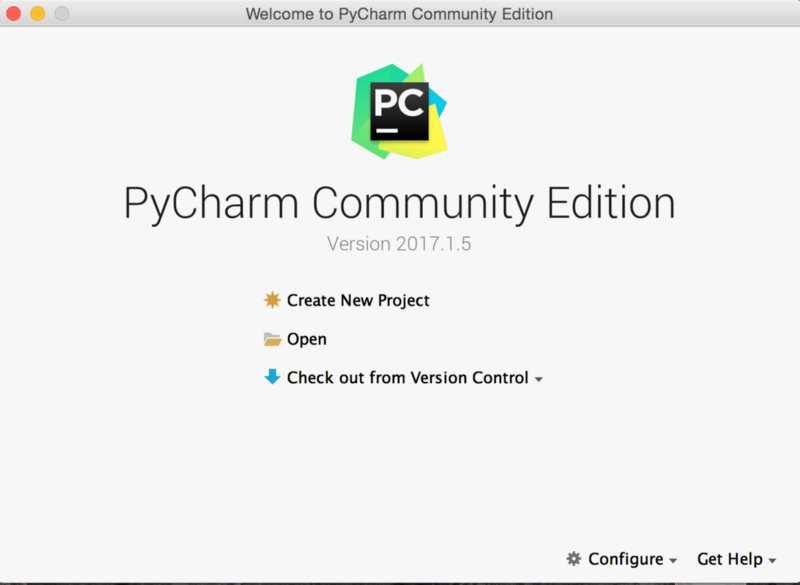
\includegraphics[width=0.7\linewidth,keepaspectratio]{pycharm2}
\end{center}
\end{frame}

%%%%%%%%%%%%%%%%%%%%%%%%%%%%%%%%%%%%%%%%%%%%%%%%%%%%%%%%%%%%%%%%%%%%%%%%%%%%%%%%%%%
\begin{frame}[fragile]\frametitle{PyCharm Exercise}

  \begin{itemize}
  \item Create a directory.
  \item Create New Project in Pychram. 
  \item Give the newly created dir as path.
  \item Create New Python file. Write:
    \begin{lstlisting}
 print(``Hello World!!'')
    \end{lstlisting}
  \item Run.
  \item Result?.
  \item Get familiar with Pycharm UI.
  \end{itemize}
\end{frame}


